\subsection{Schema Registry} \label{sec:schema_registry}
\paragraph{Documentazione} \href{https://docs.confluent.io/platform/current/schema-registry/index.html}{https://docs.confluent.io/platform/current/schema-registry/index.html} (Consultato 25/03/2024)


Schema Registry fornisce un repository centralizzato per la gestione e la convalida degli schemi relativi ai dati dei messaggi degli argomenti, nonché per la serializzazione e la deserializzazione dei dati sulla rete. I produttori e i consumatori degli argomenti Kafka possono sfruttare gli schemi per garantire la coerenza e la compatibilità dei dati mentre questi ultimi si evolvono nel tempo. Il Schema Registry rappresenta un elemento chiave per la governance dei dati, poiché contribuisce ad assicurare la qualità dei dati, la conformità agli standard, la tracciabilità dell'origine dei dati, le capacità di audit, la collaborazione tra team, protocolli di sviluppo delle applicazioni efficienti e le prestazioni del sistema.


\begin{figure}[H]
    \centering
    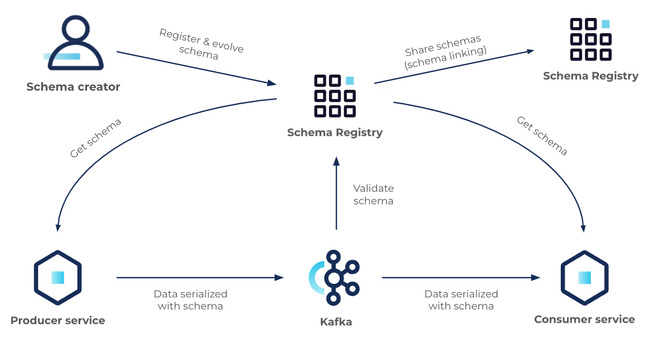
\includegraphics[width=0.9\textwidth]{../Images/SpecificaTecnica/schemaRegistry.jpg}
    \caption{Schema Registry Overview - Confluent Documentation}
    \label{fig:schemaReg}
  \end{figure}
La convalida del formato dei messaggi è un passo fondamentale per garantire l'integrità e l'affidabilità dei dati in un sistema di messaggistica come Apache Kafka. Schema Registry offre un potente strumento per la convalida dei messaggi in Kafka, fornendo diversi vantaggi:
\begin{enumerate}
    \item \textbf{Convalida dei messaggi:} Schema Registry convalida i messaggi in base allo schema registrato per il topic. I messaggi non validi vengono scartati.
    \item \textbf{Maggiore affidabilità:} La convalida dei messaggi aiuta a prevenire errori e a garantire che i dati siano conformi allo schema definito. Questo riduce il rischio di corruzione dei dati e di errori di elaborazione nei sistemi a valle.
    \item \textbf{Interoperabilità:} Schema Registry facilita la comunicazione tra diversi sistemi che producono e consumano messaggi Kafka. Definendo un formato comune per i messaggi, i sistemi possono interoperare senza problemi, anche se sono sviluppati in linguaggi di programmazione diversi o utilizzano librerie client differenti.
    \item \textbf{Evolutività:} Schema Registry permette di evolvere gli schemi dei messaggi nel tempo in modo compatibile. Ciò significa che è possibile aggiungere nuovi campi o modificare la struttura dei messaggi senza interrompere i sistemi esistenti.
    \item \textbf{Migliore debug:} La convalida dei messaggi fornisce informazioni utili in caso di errori, facilitando l'identificazione del problema e la sua risoluzione.
    \item \textbf{Sicurezza:} La convalida dei messaggi può essere utilizzata per proteggere il sistema da messaggi malformati o dannosi.
    
\end{enumerate}

Come funziona la convalida del formato dei messaggi con Schema Registry:
\begin{itemize}
    \item \textbf{Definizione dello schema:} Vengono definiti gli schemi per i messaggi Kafka utilizzando il formato JSON Schema e registrati in Schema Registry.
    \item \textbf{Produzione dei messaggi:} I producer Kafka inviano messaggi conformi allo schema definito. I messaggi possono essere inviati in topic specifici.
    \item \textbf{Convalida dei messaggi:} Schema Registry convalida i messaggi in base allo schema registrato per il topic. I messaggi non validi vengono scartati.
    \item \textbf{Consumo dei messaggi:} I consumer Kafka ricevono solo messaggi validi. I messaggi possono essere elaborati in modo affidabile dai sistemi a valle.
\end{itemize}

\subsubsection{Schema dei messaggi}\label{sec:schema_registry_sez_schema}
I messaggi nei topic dedicati allo streaming delle misurazioni dei sensori i messaggi devono essere nel seguente formato per superare la convalida definita da contratto nello Schema Registry.
\paragraph{Misurazioni dei senori}
\begin{lstlisting}[style=code]
    Da inserire
\end{lstlisting}


\paragraph{Misurazioni del punteggio di salute}
I messaggi nel topic dedicato allo streaming delle misurazioni dei punteggi di salute devono essere nel seguente formato per superare la convalida definita da contratto nello Schema Registry.
\begin{lstlisting}[style=code]
    Da inserire
\end{lstlisting}